
\clearpage{}
\section{Applications and Pragmatics}
\label{sec:performance}

In this section we discuss two end-user applications that were first written with Repa 2, and then modified to work with Repa 3 by the first author. Providing a better way to implement these applications was the reason we started this paper. The first is available in the @gloss-examples@ package, and the second in the @repa-examples@ package. Gloss is a graphics library that depends on Repa.


% -----------------------------------------------------------------------------
\subsection{Fluid Flow}
\label{section:FluidFlow}

Figure~\ref{figure:Fluid} shows output from a fluid flow solver written by Ben \mbox{Lambert-Smith}. This is an implementation of Jos Stam's stable fluid algorithm \cite{Stam:StableFluids}, which is a fast approximate algorithm intended for animation and games, rather than accurate engineering simulation. It performs a finite time-step simulation on a 2-d grid. It is numerically stable for arbitrary sized time-steps, which makes it attractive for real-time animation where the frame-rate of the simulation may vary depending on system load. We discuss the difference between the three images of Figure~\ref{figure:Fluid} in \S\ref{section:Relaxation}.

The fluid is represented as a pair of 2-d arrays, one for the density at each point, and one for the velocity. The density is a scalar floating point value, while the velocity is a 2-d vector. The majority of the runtime is spent in a function called \emph{the linear solver}, which performs matrix relaxation involving the discrete Laplace operator ($\nabla^2$). The linear solver is used to diffuse the density and velocity fields throughout the grid, as well as apply a projection operator to the velocity field, which makes it mass-preserving \cite{Stam:StableFluids}.

Our implementation of the linear solver uses Repa's support for stencil convolution, using the cursored arrays from \S\ref{section:Cursored}, and repeatedly computes the following for each grid element:
$$
u''_{i,j} = (u_{i,j} + a ~.~ (u'_{i-1,j} ~+~ u'_{i+1,j} ~+~ u'_{i,j-1} ~+~ u'_{i,j+1})) ~/~ c
$$
For each time step we perform several relaxation iterations to allow the solution to converge. In the above equation, $u$ is the grid in the previous time step, $u'$ is the grid in the current time step and the previous relaxation iteration, and $u''$ is the grid in the current time step and current iteration. The $a$ and $c$ values are constants determined by simulation parameters, such as the diffusion rate.

The linear solver is written to be polymorphic in the type of array elements. It is then specialised to 2-d vectors (for the velocity) as well as scalar floats (for the density) using GHC's specialisation pragmas \cite{PeytonJones:RewriteRules}. 


% ----------------------------------------------------------------------------
\begin{figure}
\begin{center}
\includegraphics[scale=0.75]{figs/fluid/0100-jacobi4}
\includegraphics[scale=0.75]{figs/fluid/0100-jacobi10}
\includegraphics[scale=0.75]{figs/fluid/0100-jacobi100}
\caption{Fluid Solver output for 4, 10, and 100 Jacobi iterations.}
\label{figure:Fluid}
\end{center}
\end{figure}


% ----------------------------------------------------------------------------
\subsubsection{Scheduling and Smallness Hints}
\label{section:Smallness}
In the Repa version, the linear solver is called four times: once on the scalar density field, and three times on the vector velocity field. Each time it is called, it iteratively performs 40 convolutions with the appropriate stencil, for a total of 160 convolutions per time-step. As the algorithm is intended for real-time simulation, at 30 frames (steps) per second it must perform $30 \times 160 = 4800$ convolutions per second, or one every 200 microseconds. This interval is of the same order of magnitude as the context switch latency on a typical desktop operating system \cite{Li:ContextSwitch}.

When benchmarking the fluid solver using ThreadScope~\cite{Jones:ThreadScope}, we noticed that for a grid of size $100 \times 100$ it was spending over half its time stalled while waiting for worker threads to be scheduled. For context, with a single thread, a grid of size $150 \times 150$ is about largest that will run smoothly at 30 frames per second on our desktop machine. We present concrete numbers in Figure~\ref{figure:FluidRuntime}.

\begin{figure}
\begin{center}
\includegraphics[scale=0.2]{data/fluid/par}
\hspace{2em}
\includegraphics[scale=0.2]{data/fluid/seq}
\end{center}
\caption{Fluid Thread Activity}
\label{figure:FluidActivity}
\end{figure}

% -----------------------------------------------
\begin{figure}
\begin{small}
\begin{code}
data S r
instance Source (S r) sh e
 data Array (S r) sh e 
        = HintSmall (Array r sh e)
 ...

instance ( Shape sh, Load r sh e) 
        => Load (S r) sh e where
 loadP (HintSmall arr) marr = loadS arr marr
 loadS (HintSmall arr) marr = loadS arr marr

type PS5 = P C (P (S D) (P (S D) (P (S D) (P (S D) X))))
mapStencil2 :: Source r DIM2 a 
  => Boundary a     -> Stencil DIM2 a
  -> Array r DIM2 a -> Array PS5 DIM2 a
\end{code}
\end{small}
\caption{Smallness Hints}
\label{figure:SmallnessHints}
\end{figure}


The left of Figure~\ref{figure:FluidActivity} is a ThreadScope plot for the $100 \times 100$ version showing the problem. This plot was taken on an $2\times$QuadCore Intel Harpertown server running Linux Kernel 2.6.32. To minimise the chance of our benchmark being interrupted by the operating system, it was run with only 7 threads (out of 8 possible), leaving the final core for the OS. We use thread affinity to bind each Haskell thread to a single core. In the figure, the 7 horizontal traces show the period each thread was active. The graph at the top shows how many threads were active at each point in time. 

The graph shows two bursts of high activity where the benchmark was performing a matrix relaxation step, and the start of a third one on the far right hand side. As mentioned in \S\ref{section:FluidFlow}, the matrix relaxation is performed using a stencil convolution, which uses the partitioned array representation from \S\ref{section:Partitioned}. Each burst of high activity, where the plot shows all seven threads active, corresponds to the computation of the \emph{inner} region of the array. The four short bursts after it correspond to the computation of the border regions. Because computation of a border region is so little work, more time is spent waiting for the computation to be scheduled than actually computing it.

We address this problem with \emph{smallness hints}, which are wrappers for Repa's usual Delayed (@D@) and Cursored (@C@) type indices. The definition is given in Figure~\ref{figure:SmallnessHints}. Whereas the application of @computeP@ from \S\ref{section:Partitioned} to an array of type @Array D DIM2 Int@ will proceed in parallel, application to an @Array (S D) DIM2 Int@ will proceed sequentially. This behaviour is straightforward to add to our existing framework, as the evaluation method for each array representation is given by the corresponding instance of the @Load@ class. Given some inner representation @r@, the @Load@ instance for @S r@ simply redirects applications of both @loadP@ and @loadS@ to the @loadS@ method for @r@. 

We force the borders of a partitioned array to be evaluated sequentially by modifying the definition of @mapStencil2@ from \S\ref{section:Partitioned}. All that is needed is to wrap the existing border definition in the @HintSmall@ constructor. The effect on the type of @mapStencil2@ is also shown in Figure~\ref{figure:SmallnessHints}.

The ThreadScope plot in the right of Figure~\ref{figure:FluidActivity} is for the same benchmark, now using smallness hints for the border partitions. Now only the main thread is active between each high-activity burst, yet the period of low activity is shorter. 

There is a design choice about whether to preserve smallness hints in the result of an @smap@ operation \S\ref{section:Structured}. Although computation of a particular region in a delayed array may correspond to a small amount of work, after we map a function across every element, computation of the same region in the result may be more expensive. For now we arrange @smap@ to preserve the smallness hint in the result array, though we will return to this in \S\ref{section:HintInteraction}.


% ----------------------------------------------------------------------------
\subsubsection{Gauss-Seidel vs Jacobi relaxation}
\label{section:Relaxation}
The reference C implementation of Jos Stam's fluid flow algorithm was supplied with \cite{Stam:StableFluids}. The linear solver in this version uses Gauss-Seidel matrix relaxation while we use Jacobi relaxation. Relative to the equation in \S\ref{section:FluidFlow}, Gauss-Seidel relaxation replaces the $u'_{i-1,j}$ and $u'_{i,j-1}$ terms with $u''_{i-1,j}$ and $u''_{i,j-1}$ respectively. In the reference version these array elements are read from the array currently being written to. Jacobi relaxation uses the equation as written. 

Although the ``fast forwarding'' of array elements in Gauss-Seidel reduces the number of iterations needed to achieve convergence, its use of destructive update makes it difficult to parallelise. Destructive update also causes problems for optimising compilers such as LLVM (which GHC uses for back-end compilation) as they must worry about potential aliasing between the source and result arrays. In contrast, Jacobi relaxation is kinder to optimising compilers, and easier to parallelise, but requires more iterations than Gauss-Seidel as it does not converge as fast.

For Stam's algorithm, the penalty for using an insufficient number of iterations is an unattractive image with too much numerical dissipation \cite{Stam:StableFluids}. Figure~\ref{figure:Fluid} shows the result of simulating 100 time steps from identical initial conditions, using 4, 10 and 100 Jacobi iterations in the linear solver. For low iteration counts, the swirls present in the right-most image do not appear in the output.

To ensure a fair comparison, our Repa implementation using Jacobi relaxation must use more iterations than the reference implementation. We determined an appropriate number by first simulating the initial conditions used in Figure~\ref{figure:Fluid} using 1000 Gauss-Seidel iterations, treating this as the ideal output. We then measured the mean-square error between the ideal output, and the output using 20 Gauss-Seidel iterations, which is what Stam's reference implementation uses. Finally, we increased the number of Jacobi iterations until the error in the output was reduced to the same level as the reference version. Using 38 Jacobi iterations achieves the same error figure, which we round up to 40 for good measure.



% -----------------------------------------------------------------------------
\subsubsection{Comparison}
Figure~\ref{figure:FluidRuntime} shows the relative runtimes between Stam's C implementation using Gauss-Seidel relaxation (with 20 iterations), and the same program modified to use Jacobi relaxation (with 40 iterations). We also show relative runtime for the Repa version using Jacobi relaxation with 1, 2 and 4 threads. 

The overall shape of this plot is as we would expect. At small array sizes the sequential C versions are faster as they preallocate buffers for the source and result arrays, and swap them after every iteration. This improves data locality, reducing the cache miss rate. In contrast, the Repa version allocates a fresh result buffer for every iteration, leaving old buffers to be reclaimed by the garbage collector. 

At large array sizes, the working set no longer fits in cache and the single threaded Repa Jacobi solver is faster than the C version. This is because cursored arrays allows the Repa version to share intermediate computations, which reduces overall instruction count and memory bandwidth. For large array sizes the benchmark is memory bound, so performance does not scale linearly with an increased number of threads. 

The C reference implementation could be improved by hand-applying the unroll-and-jam transformation that is baked into the Repa library. We tried various permutations of @-funroll-loops@ when compiling with GCC 4.2.1, but inspection of the assembly output revealed it was not recovering the same inter-stencil sharing as the Repa version due to aliasing problems --- even though the loops were indeed unrolled. Compiling with Clang 3.0 (which uses LLVM for the backend) did not significantly improve matters. On the other hand, we could also improve the Repa version by preallocating the source and result arrays and using the @ForeignPtr@ support to swap and reuse the same buffers between iterations.


\begin{figure}
% GNUPLOT: LaTeX picture with Postscript
\begingroup
  \makeatletter
  \providecommand\color[2][]{%
    \GenericError{(gnuplot) \space\space\space\@spaces}{%
      Package color not loaded in conjunction with
      terminal option `colourtext'%
    }{See the gnuplot documentation for explanation.%
    }{Either use 'blacktext' in gnuplot or load the package
      color.sty in LaTeX.}%
    \renewcommand\color[2][]{}%
  }%
  \providecommand\includegraphics[2][]{%
    \GenericError{(gnuplot) \space\space\space\@spaces}{%
      Package graphicx or graphics not loaded%
    }{See the gnuplot documentation for explanation.%
    }{The gnuplot epslatex terminal needs graphicx.sty or graphics.sty.}%
    \renewcommand\includegraphics[2][]{}%
  }%
  \providecommand\rotatebox[2]{#2}%
  \@ifundefined{ifGPcolor}{%
    \newif\ifGPcolor
    \GPcolorfalse
  }{}%
  \@ifundefined{ifGPblacktext}{%
    \newif\ifGPblacktext
    \GPblacktexttrue
  }{}%
  % define a \g@addto@macro without @ in the name:
  \let\gplgaddtomacro\g@addto@macro
  % define empty templates for all commands taking text:
  \gdef\gplbacktext{}%
  \gdef\gplfronttext{}%
  \makeatother
  \ifGPblacktext
    % no textcolor at all
    \def\colorrgb#1{}%
    \def\colorgray#1{}%
  \else
    % gray or color?
    \ifGPcolor
      \def\colorrgb#1{\color[rgb]{#1}}%
      \def\colorgray#1{\color[gray]{#1}}%
      \expandafter\def\csname LTw\endcsname{\color{white}}%
      \expandafter\def\csname LTb\endcsname{\color{black}}%
      \expandafter\def\csname LTa\endcsname{\color{black}}%
      \expandafter\def\csname LT0\endcsname{\color[rgb]{1,0,0}}%
      \expandafter\def\csname LT1\endcsname{\color[rgb]{0,1,0}}%
      \expandafter\def\csname LT2\endcsname{\color[rgb]{0,0,1}}%
      \expandafter\def\csname LT3\endcsname{\color[rgb]{1,0,1}}%
      \expandafter\def\csname LT4\endcsname{\color[rgb]{0,1,1}}%
      \expandafter\def\csname LT5\endcsname{\color[rgb]{1,1,0}}%
      \expandafter\def\csname LT6\endcsname{\color[rgb]{0,0,0}}%
      \expandafter\def\csname LT7\endcsname{\color[rgb]{1,0.3,0}}%
      \expandafter\def\csname LT8\endcsname{\color[rgb]{0.5,0.5,0.5}}%
    \else
      % gray
      \def\colorrgb#1{\color{black}}%
      \def\colorgray#1{\color[gray]{#1}}%
      \expandafter\def\csname LTw\endcsname{\color{white}}%
      \expandafter\def\csname LTb\endcsname{\color{black}}%
      \expandafter\def\csname LTa\endcsname{\color{black}}%
      \expandafter\def\csname LT0\endcsname{\color{black}}%
      \expandafter\def\csname LT1\endcsname{\color{black}}%
      \expandafter\def\csname LT2\endcsname{\color{black}}%
      \expandafter\def\csname LT3\endcsname{\color{black}}%
      \expandafter\def\csname LT4\endcsname{\color{black}}%
      \expandafter\def\csname LT5\endcsname{\color{black}}%
      \expandafter\def\csname LT6\endcsname{\color{black}}%
      \expandafter\def\csname LT7\endcsname{\color{black}}%
      \expandafter\def\csname LT8\endcsname{\color{black}}%
    \fi
  \fi
  \setlength{\unitlength}{0.0500bp}%
  \begin{picture}(5040.00,3310.00)%
    \gplgaddtomacro\gplbacktext{%
      \csname LTb\endcsname%
      \put(472,496){\makebox(0,0)[r]{\strut{} 0}}%
      \put(472,992){\makebox(0,0)[r]{\strut{} 0.5}}%
      \put(472,1489){\makebox(0,0)[r]{\strut{} 1}}%
      \put(472,1985){\makebox(0,0)[r]{\strut{} 1.5}}%
      \put(472,2482){\makebox(0,0)[r]{\strut{} 2}}%
      \put(472,2978){\makebox(0,0)[r]{\strut{} 2.5}}%
      \put(604,276){\makebox(0,0){\strut{}64}}%
      \put(1179,276){\makebox(0,0){\strut{}96}}%
      \put(1587,276){\makebox(0,0){\strut{}128}}%
      \put(2162,276){\makebox(0,0){\strut{}192}}%
      \put(2570,276){\makebox(0,0){\strut{}256}}%
      \put(3144,276){\makebox(0,0){\strut{}384}}%
      \put(3552,276){\makebox(0,0){\strut{}512}}%
      \put(4127,276){\makebox(0,0){\strut{}768}}%
      \put(4535,276){\makebox(0,0){\strut{}1024}}%
      \put(0,1737){\rotatebox{-270}{\makebox(0,0){\strut{}relative runtime}}}%
      \put(2569,50){\makebox(0,0){\strut{}matrix width}}%
      \put(669,1588){\makebox(0,0)[l]{\strut{}C Gauss-Seidel}}%
      \put(669,1141){\makebox(0,0)[l]{\strut{}C Jacobi}}%
      \put(3777,1737){\rotatebox{-10}{\makebox(0,0)[l]{\strut{}Repa -N1}}}%
      \put(3777,1370){\rotatebox{-10}{\makebox(0,0)[l]{\strut{}Repa -N2}}}%
      \put(3777,943){\rotatebox{-10}{\makebox(0,0)[l]{\strut{}Repa -N4}}}%
    }%
    \gplgaddtomacro\gplfronttext{%
    }%
    \gplbacktext
    \put(0,0){\includegraphics{data/fluid/tesla-size}}%
    \gplfronttext
  \end{picture}%
\endgroup

\caption{Runtimes for Fluid Flow Solver}
\label{figure:FluidRuntime}
\end{figure}


% -----------------------------------------------------------------------------
\subsection{Unbalanced Workloads}
\label{section:Unbalanced}
Figure~\ref{figure:UnbalancedImages} shows three example applications with unbalanced workloads, all written with Repa. The first is a Mandelbrot set visualisation computed with the escape-time algorithm. In the output image, the pixels in the (approximate) Mandelbrot set are rendered black and take about 10 times longer to compute than the others.


% -----------------------------------------------------------------------------
\begin{figure}
\begin{center}
\includegraphics[scale=0.3]{figs/mandel/mandel-lightened}\\
\includegraphics[scale=0.3]{figs/ray/ray-lightened}\\
\includegraphics[scale=0.3]{figs/spline/spline-montage}
\caption{Unbalanced Workloads}
\label{figure:UnbalancedImages}
\end{center}
\end{figure}

The second is output from a real-time ray tracer, where parts of the image showing many reflections take longer to compute than the others. Although ray tracing is known in the folklore as ``embarassingly parallel'' as every pixel in the output can be computed independently, it is not embarrassingly \emph{data parallel} due to the unbalanced workload.

The final example is an interpolator for volumetric data, which implements the algorithm described in \cite{Sorokina:Spline}. This example was written by Michael Orlitzky using Repa 2, and then modified to work with Repa 3 by the first author. The left-most image at the bottom of Figure~\ref{figure:UnbalancedImages} shows one slice though a $256 \times 256 \times 109 \times 16$-bit data volume from a Magnetic Resonance Imaging (MRI) machine. The bottom-center image is from the source data, and shows a scaled region of the top-right portion of the brain. The bottom-right image shows the same region after interpolation. In a straightforward implementation, every element in the output volume is computed independently and takes the same amount of time. However, we can improve the overall runtime by returning a constant zero value (black pixel) for voxels corresponding to the air surrounding the physical object. This is done by summing the surrounding voxels in the source data, and testing the sum against a user defined threshold. This is faster than calculating the true interpolated result, but again makes the workload unbalanced.


% -----------------------------------------------------------------------------
\subsubsection{Spacial Correlation and Interleaved Evaluation}
\label{section:Interleaved}
The workloads of our three examples are unbalanced because the cost to compute each array element is not uniform throughout the array. The standard Repa evaluation method chunks the underlying row-major vector evenly between the available threads. When using cursored arrays we instead proceed column-wise as this is more cache-efficient when performing convolutions on 2-d matrices. The figure below shows both of these methods, assuming we are computing the matrix with three threads.
%
\begin{center}
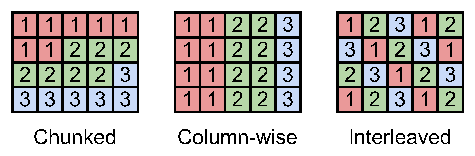
\includegraphics[scale=0.8]{figs/guiding-eval-order}
\end{center}
%
With both the Chunked and Column-wise method, the spacial correlation between features in the result array, and computational workloads maps directly onto the physical processors. The left of Figure~\ref{figure:InterpolatorThreads} is a ThreadScope plot that shows the effect of this correlation in sharp relief. The plot is for the interpolator on seven threads, which shows the threads that compute non-zero data in the result take significantly longer to run. The plot is for the entire run of the program, and the high-activity bursts at the beginning and end are due to reading source data and writing the output to file.

A well known solution to this problem is to move to an interleaved evaluation method instead \cite{Salmon:RayTracer}, also shown in the figure above. When applied to ray tracing this approach is classically known as \emph{image space partitioning} to distinguish it from \emph{object space partitioning} which divides the model being rendered. As with all static load-balancing strategies, there is still a chance that the runtime-workload will correlate with the assigned thread index, though this would be unlikely for the three applications shown in Figure~\ref{figure:UnbalancedImages}. Lee and Raghavendra~\cite{Lee:RayTracerLoadBalancing} compare related strategies. 

\begin{figure}
\begin{center}
\includegraphics[scale=0.25]{data/spline/spline3-unbalanced}
\hspace{3em}
\includegraphics[scale=0.25]{data/spline/spline3-interleave}\\
\caption{Interpolator Thread Activity}
\label{figure:InterpolatorThreads}
\end{center}
\end{figure}

We implement our new interleaved evaluation method similarly to the smallness hints from \S\ref{section:Smallness}, with the main definitions given Figure~\ref{figure:InterleaveHints}. Whereas application of @computeP@ to an array of type @Array D DIM2 Int@ will use chunked evaluation, application to an @Array (I D) DIM2 Int@ now uses interleaved evaluation, implemented by @fillInterleavedP@. The right of Figure~\ref{figure:InterpolatorThreads} shows the result of using interleaved evaluation for the interpolator. All threads now run for approximately the same period of time, and of the overall runtime of the program is shorter. 

% Note that although interleaved evaluation causes different threads to write to alternate elements, this does not in itself cause serious cache contention. The first time one thread tries to write to a cache line owned by another it will be stalled. This allows time for the second thread to advance further, which reduces the likelihood of a subsequent conflict. We verified the lack of cache-contention by integrating the thread activity plots for out three benchmarks over time. The total workload (in units of thread-seconds) is identical for interleaved and non-interleaved evaluation, for each benchmark. 


% -----------------------------------------------------------------------------
\begin{figure}
\begin{small}
\begin{code}
data I r1
instance Source (I r1) sh e
 data Array (I r1) sh e
        = HintInterleave (Array r1 sh e)

instance ( Shape sh, Load D sh e) 
        => Load (I D) sh e where
 loadP (HintInterleave (ADelayed sh getElem)) marr 
   = fillInterleavedP (size sh) (unsafeWriteMArr marr) 
                                (getElem . fromIndex sh) 
 loadS (HintInterleave arr) marr = loadS arr marr

instance Structured rs a => Structured (I rs) a where
 type TR (I rs) = I (TR rs)
 ...
\end{code}
\end{small}
\caption{Interleave Hints}
\label{figure:InterleaveHints}
\end{figure}


% -----------------------------------------------------------------------------
\subsubsection{Hint Propagation and Interaction}
\label{section:HintInteraction}
The @Load@ instance in Figure~\ref{figure:InterleaveHints} only works for Delayed (@D@) arrays, and not Cursored (@C@) arrays as well. As described in \S\ref{section:Cursored}, cursored arrays are used to share intermediate computations between adjacent array elements, and this process depends on a particular traversal order. As adjacent elements must be computed in the same loop iteration, using interleaved evaluation with cursored arrays would be of no benefit.

Smallness hints and interleave hints interact in a natural way. If a delayed array is wrapped in an Interleave (@I@) hint, this signals that its parallel computation will be unbalanced. If it is then wrapped in a Smallness (@S@) hint as well, this signals that it is a small amount of work \emph{relative} to some larger computation. The combination of hints yields a type index of @(S (I D))@. When the array is finally computed, the instances given in Figures \ref{figure:SmallnessHints} and \ref{figure:InterleaveHints} effectively ignore the interleave hint, as the sequential evaluation enforced by smallness cannot itself be unbalanced. If the two hints are applied in the other order, to yield an index of @(I (S D))@ then there is no available @Load@ instance, because hinting that a sequential computation is unbalanced does not make sense.

Finally, note that the @Structured@ instance in Figure~\ref{figure:InterleaveHints} propagates the interleave hint to the result representation. The declaration of @Structured@ was given in Figure~\ref{figure:Structured}. We preserve this hint because the @Structured@ class methods, namely @smap@ and @szipWith@ are bulk operations, meaning they apply the same function to every array element. In practice, it is highly unlikely that applying such an operation to an array defining an unbalanced workload would make it \emph{more} balanced, so it is better to retain the unbalancedness. For example, suppose we apply our ray-tracer to a 3d model and then convert the output image to greyscale:
%
\begin{small}
\begin{code}
  image :: Array U DIM2 Float
  image = computeP $ smap toGreyScale $ raytrace model
\end{code}
\end{small}
%
The result of evaluating @raytrace model@ will have the type \\ @Array (I D) DIM2 (Float, Float, Float)@, where the tuple contains red, green, blue color values. Applying @smap toGreyScale@ the produces @Array (I D) DIM2 Float@, where the result gives a luminance value for each pixel. The array defined by the @raytrace@ is unbalanced, and when fused with @toGreyScale@ it remains unbalanced. 


